
\section{Kitaev's Honeycomb Model}

Let us begin by providing a review of the model as it was originally proposed by Kitaev in \cite{kitaev_anyons_2006}. We shall present the spin Hamiltonian, as well as the Majorana transformation used to diagonalise it. Following this, we shall discuss the ground-state phase diagram and finally the presence of anyonic excitations. In \textsection\ref{sec:amorphous_kitaev_model}, we will describe the amorphous version of this model, generalised to arbitrary lattice geometry. Thus, the methods will be presented in a language that allows for a straightforward generalisation to different lattice geometry. 
\begin{figure} 
    \begin{center}
        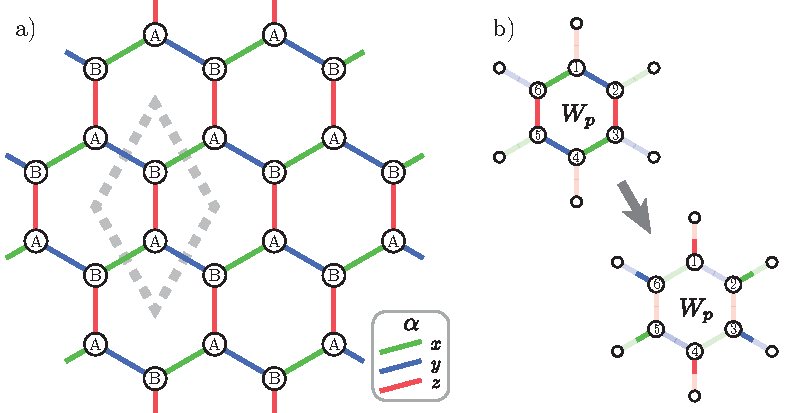
\includegraphics[]{kitaev_model/figures/honeycomb_kit.pdf}
        \caption{
            \textbf{(a)} A section of honeycomb lattice with the bond labels shown according to colour. The unit cell is marked by the dashed grey rhombus.
            \textbf{(b)} A single $W_p$ operator, where the full-colour lines indicate the bond operators that take part in $W_p$. After multiplying out the Pauli operators, the remaining terms are shown, corresponding to spin operators that connect outwards from the plaquette. States are numbered to correspond to the ordering in eqn.~\ref{eqn:wp_operator}.
        }\label{fig:honeycomb_kitaev}
    \end{center}
\end{figure}

The Kitaev honeycomb model is defined for a set of spin half degrees of freedom on the vertices of a honeycomb lattice, as shown in fig.~\ref{fig:honeycomb_kitaev}a. The bonds in this lattice are labelled with an index $\alpha \in \{x, y, z\}$, such that each site connects to one bond of each type. On each bond, neighbouring spins interact with a bond-directional Ising-type coupling. The Hamiltonian is given by
\begin{align}
    H = -J^x \sum_{x\textup{-bonds}} \sigma_j^x \sigma_k^x
    -J^y \sum_{y\textup{-bonds}} \sigma_j^y \sigma_k^y
    -J^z \sum_{z\textup{-bonds}} \sigma_j^z \sigma_k^z,
\end{align}
where the parameters $J^\alpha$ determine the strength of the $x$, $y$ and $z$ bonds, and $\sigma_j^\alpha$ represents a Pauli operator acting on the spin at site $j$. The exact solution of this model -- as with all integrable systems --  depends on the presence of an extensive set of conserved quantities, given by the following $W_p$ operators, defined by taking the product of the bond operators around a given hexagonal plaquette, $p$, 
\begin{align}
    W_p = \sum_{\braket{jk} \in p}
    \sigma_j^\alpha \sigma_k^\alpha,
\end{align}
where the order of the $\sigma_j$ operators is arranged such that they run clockwise around the hexagonal plaquette. Using that standard Pauli multiplication rules, we can show that the product can be simplified into a product of the six Pauli operators that connect outwards from each site on the hexagon. For example, the plaquette shown in fig.~\ref{fig:honeycomb_kitaev}b has $W_p$ given by
\begin{align} \label{eqn:wp_operator}
    W_p = \sigma^z_1 \sigma^x_2 \sigma^y_3
    \sigma^z_4 \sigma^x_5 \sigma^y_6
\end{align} 
All $W_p$ operators commute with each other and $H$. Furthermore, we have $W_p^2 = 1$, which means that $W_p$ have eigenvalues $\pm 1$. The Hilbert space has dimension $2^N$, where $N$ is the number of spins. Since we have $N/2$ plaquettes in the system, these conserved quantities allow us to split the Hilbert space into $2^{N/2}$ sectors according to the eigenvalues of $\{W_p\}$.

\subsection{Spins to Fermions to Majoranas}

Although the Kitaev model can be solved with a Jordan-Wigner transformation \cite{feng_topological_2007,chen_exact_2007,chen_exact_2008}, here we will follow the original construction in terms of Majorana fermions. The first step is an old trick, often referred to as the parton construction \cite{senthil_z2_2000, wen_theory_1996, wen_quantum_2007}. We introduce a pair of fermion operators for each site, $f^\dag_\uparrow$ and $f^\dag_\downarrow$, which create a spin up and spin down state respectively. Spin operators are straightforwardly modified to
\begin{align}
    \sigma^\alpha \rightarrow f^\dag _{\mu} \sigma^\alpha_{\mu \nu} f_\nu.
\end{align}
In performing this transformation we have artificially enlarged our Hilbert space, since each site can now host four states. Two of these states are the original spin up and down states, forming part of the physical Hilbert space $\mathcal H_{\textup{phys}}$. The other two correspond to no spin at all, or both a spin up and spin down on a single site. These states form the unphysical auxiliary Hilbert space $\mathcal H_{\textup{aux}}$.
\begin{center}
    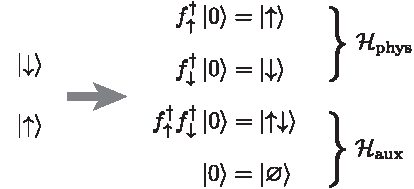
\includegraphics[scale=1.1]{kitaev_model/figures/hilbert_space_fermions.pdf}
\end{center}
Thus, we can construct a parity operator that determines whether a state is in the physical or auxiliary Hilbert space using a product over fermionic number operators on a single site, $ n_{j\mu} = f^\dag_{j \mu} f_{j \nu}$,
\begin{align}
    D_{j} = -(1 - 2 n_{j\uparrow})(1 - 2 n_{j\downarrow}).
\end{align}
This operator has the property that $D_j \ket \psi = + (-)\ket \psi$ for states in the physical (auxiliary) Hilbert space. Next let us decompose each fermion into a pair of Majorana fermions according to the following substitution,
\begin{align}
    f_\downarrow &= \frac{1}{2} (c + i b^z), \\ 
    f_\uparrow &= \frac{1}{2} (b^y + i b^x),
\end{align}
where the Majorana operators have standard Majorana commutation relations,
\begin{align}
    c^\dag = c,\qquad \{c_j , c_k \} = 2\delta_{jk},
\end{align}
with the same relations for $b$-type Majoranas. In this new formalism, a fermionic parity operator becomes
\begin{align}
    i c b^z = 2 f_\downarrow ^\dag f_\downarrow - 1,
\end{align}
with the corresponding identity for $f_\uparrow$ using $b^y$ and $b^x$. Thus, the parity operator $D$ becomes
\begin{align}
    D =  b^x b^y b^z c.
\end{align}
In the Majorana representation, the spin operators take the following form,
\begin{align}
    \sigma^x  & \rightarrow \frac{i}{2} (c b^x - b^z b^y), \\ 
    \sigma^y  & \rightarrow \frac{i}{2} (c b^y + b^z b^x), \\ 
    \sigma^z  & \rightarrow \frac{i}{2} (c b^z - b^y b^x).
\end{align}
We're almost there, however we have one more condition to make, which is that we are acting only on states in the physical subspace -- satisfying $D \ket \psi = \ket \psi$. First let's check that the spin operators preserve the physical subspace. $D$ anti-commutes with any single Majorana operator, $\{c_j , D\} = 0$, thus $D$ commutes with any product of two Majoranas $[c_jc_k, D] = 0$. 

As long as a state is in the physical Hilbert space, we have that $c b^z b^y b^x \ket \psi = \ket \psi$ -- which can then rearranged into the following identity,
\begin{align}
    c b^z \ket \psi &= - b^y b^x \ket \psi,
\end{align}
with an equivalent identity for any other pairing of the Majoranas. Thus we see that when acted {\it only on the physical subspace} the spin operators may be represented with
\begin{align}
    \sigma^x = i c b^x,\qquad  \sigma^y = i c b^y ,\qquad  \sigma^z = i c b^z.
\end{align}

\subsection{The Majorana Hamiltonian}


\section{The Amorphous Honeycomb Model} \label{sec:amorphous_kitaev_model}
Here we write down the Kitaev Hamiltonian for a general lattice. Talk about spins, classical frustration and discuss the properties of this model.

How many conserved quantities are there, show the form of the plaquette operators and explain why they are conserved. Discuss how much this chops the Hilbert space - in general you would want a system that scales linearly with size but we're still exponential in $2^{n/2}$.


\subsection{Solving the Hamiltonian}

Now explain the process for actually solving the Hamiltonian
\begin{itemize}
    \item Describe the old XG wen trick of turning a spin into two fermions
    \item Talk about how we have doubled the Hilbert space
    \item discuss how we have to also enforce a projector onto the smaller Hilbert space
    \item Now break these fermions up into Majorana fermions
    \item Show how the spin operators become $icb$ operators in this representation
    \item Show what the projector becomes in this basis
    \item Discuss gauge invariance w/ proof
\end{itemize}

\subsection{The Ground State Phase Diagram}

\subsection{Solving the Quadratic Hamiltonian}


\subsection{Physical Realisations}